%%
% This is an Overleaf template for presentations
% using the TUM Corporate Desing https://www.tum.de/cd
%
% For further details on how to use the template, take a look at our
% GitLab repository and browse through our test documents
% https://gitlab.lrz.de/latex4ei/tum-templates.
%
% The tumbeamer class is based on the beamer class.
% If you need further customization please consult the beamer class guide
% https://ctan.org/pkg/beamer.
% Additional class options are passed down to the base class.
%
% If you encounter any bugs or undesired behaviour, please raise an issue
% in our GitLab repository
% https://gitlab.lrz.de/latex4ei/tum-templates/issues
% and provide a description and minimal working example of your problem.
%%


\documentclass[
  english,            % define the document language (english, german)
  aspectratio=169,    % define the aspect ratio (169, 43)
  % handout=2on1,       % create handout with multiple slides (2on1, 4on1)
  % partpage=false,     % insert page at beginning of parts (true, false)
  % sectionpage=true,   % insert page at beginning of sections (true, false)
]{tumbeamer}

% presentation metadata
\title{MLMC Seminar}
\subtitle{Efficient White Noise Sampling and Coupling for\\ Multilevel Monte Carlo with Nonnested Meshes}
\author{Federico Riva}

\institute{Department of Mathematics\\\theUniversityName}
\date[18 June 2026]{18 June 2026}

\footline{\insertauthor~|~\insertshorttitle~|~\insertshortdate}

\usepackage{hyperref}
\usepackage{fontawesome5}
\hypersetup{colorlinks=true,linkcolor=blue,urlcolor=blue}

\TUMbeamersetup{
  title page = TUM centered,
  part page = TUM toc,
  section page = TUM toc,
  content page = TUM more space,
  tower scale = 1.0,
  headline = TUM empty,
  footline = TUM default,
  headline on = {title page},
  footline on = {every page, title page=false},
}

% load additional packages
\usepackage{booktabs}
\usepackage{amsthm, amsmath, amssymb, bbm}
\usepackage{graphicx} 
\usepackage{algorithm2e}
\SetKwInput{KwInit}{Initialize}
\usepackage{xcolor}

\usepackage[style=authoryear, natbib=true, bibstyle=authoryear, backend=biber,
  maxcitenames=2, doi=false, isbn=false, url=false, eprint=false, date=year]{biblatex}
\DeclareDelimFormat[parencite]{finalnamedelim}{\addspace\&\space}
\addbibresource{mylibrary.bib}

\begin{document}

\maketitle

% -----------------------------------------------------------------------
\section{Introduction}
% -----------------------------------------------------------------------

\begin{frame}{Abstract}
\begin{itemize}
\item In many applications it is required to generate samples from specific points of a Gaussian
random field.
\bigskip
\item This produces a Gaussian random vector with specific distribution parameters, namely the mean vector and the covariance matrix.
\bigskip
\item Algorithms like Box-Muller let us easily sample from a standard normal distribution.
\bigskip
\item While the desired mean can be achieved via the summation of the mean vector, the right covariance is considerably more involved since it requires an expensive \textbf{Cholesky factorization}.
\end{itemize}

\end{frame}

\begin{frame}{}
\bigskip
\begin{itemize}
\bigskip
\bigskip
\item  In the particular case presented by this article the covariance matrix is the \textbf{mass matrix of a finite element method}
\bigskip
\item The main idea to make the sampling more
efficient is to exploit the assembling of the global mass matrix as a linear combination of
all mass matrices associated to each element of the mesh.
\bigskip
\item Due to linearity it is possible to
factorize the smaller mass matrices of the elements instead of the more extended global one.
\end{itemize}

\end{frame}

% -----------------------------------------------------------------------
\section{The Article}
% -----------------------------------------------------------------------

\begin{frame}{Problem Setting}

Given the following elliptic PDE with random coefficient $u$:
\begin{equation}
  \begin{cases}
    -\nabla \cdot \bigl(e^{u(x,\omega)}\,\nabla q(x,\omega)\bigr) = 1,
      & x \in G = [-0.5,\,0.5]^d,\quad \omega \in \Omega \\[4pt]
    q(x,\omega) = 0,
      & x \in \partial G,\quad \omega \in \Omega
  \end{cases}
\end{equation}

\bigskip
We are interested in estimating the expected value of the $L^2$-norm of the solution $q$:
\begin{equation}
  \mathbb{E}\!\left[\|q\|_{L^2(G)}\right]
  = \int_\Omega \|q\|_{L^2(G)}(\omega)\,d\mathbb{P}(\omega)
\end{equation}

\bigskip
This task can be also seen as computing the expected value of a real-valued random variable
\[ \mathcal{P} := \|q\|_{L^2(G)} : \Omega \to \mathbb{R}.\]

\end{frame}

% -----------------------------------------------------------------------

\begin{frame}{Mat\'ern Covariance}
Assume $u$ is a Gaussian random field with zero mean and Mat\'ern covariance $\mathcal{C}$:
\begin{equation}
  \mathcal{C}(x,y) = \frac{\sigma^2}{2^{\nu-1}\Gamma(\nu)}(\kappa r)^\nu K_\nu(\kappa r),
  \quad r = \|x-y\|_2,\quad \kappa = \frac{\sqrt{8\nu}}{\lambda},\quad x,y \in D
\end{equation}
where $\sigma^2,\nu,\lambda > 0$ are respectively the variance, smoothness and correlation length while $K_\nu$ is the modified Bessel function of second kind.
\begin{figure}[htbp]
    \centering
    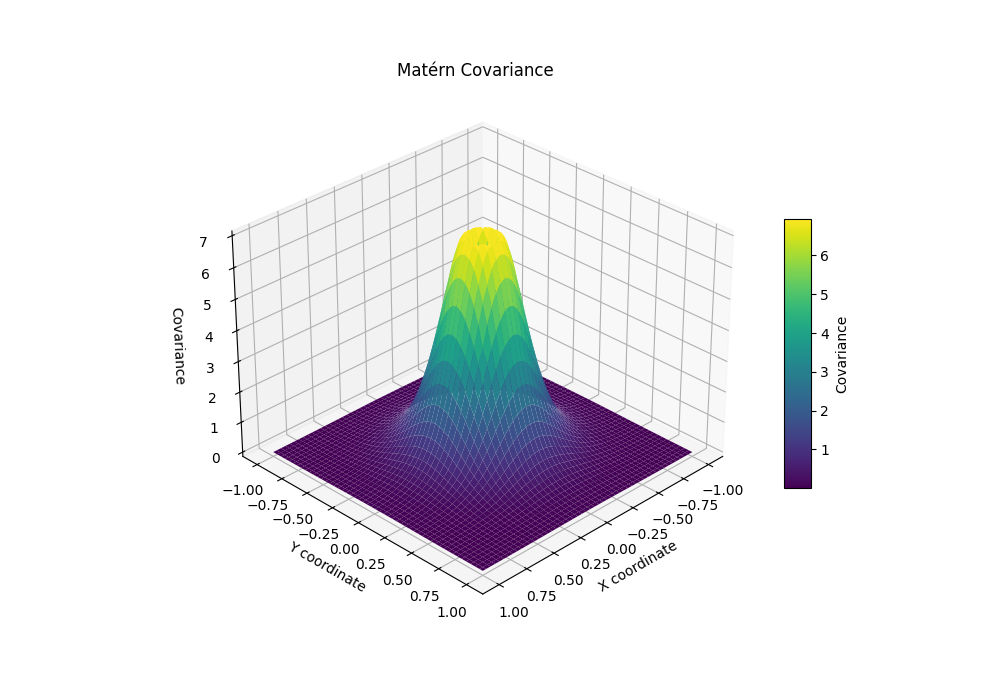
\includegraphics[width=0.5\textwidth]{images/matern_covariance_1.png}
    \label{fig:mat_cov} % Etichetta per fare riferimenti nel testo
\end{figure}
\end{frame}

\begin{frame}{Discrete Sampling}

\bigskip
In practice, samples of $u$ are needed only at discrete locations $x_1,\dots,x_m \in D$. 

\bigskip
A simple sampling strategy consists of drawing realisations of a Gaussian vector \( V\) in \( \mathbb{R}^m \)
\[ u \sim \mathcal{N}(0,C) \ \text{with} \ u_i = u(x_i) \ \text{ and covariance matrix} \ C_{ij} = \mathbb{E}[u(x_i)\,u(x_j)] \in \mathbb{R}^{m\times m}.\]
Then using Box-Muller to sample $\mathbf{z} \sim \mathcal{N}(0,I)$, $I \in \mathbb{R}^{n\times n}$, and the factorization $C = HH^T$, $H \in \mathbb{R}^{m\times n}$, gives $u = Hz$ since:
\begin{equation}
  \mathbb{E}[uu^T] = \mathbb{E}[Hz(Hz)^T]
  = H\,\mathbb{E}[zz^T]\,H^T = HIH^T = C
\end{equation}
This approach requires the factorization of a dense covariance matrix:
complexity $\mathcal{O}(m^3)$.
\end{frame}

% -----------------------------------------------------------------------

\begin{frame}{An alternative Sampling Method: the SPDE Approach}

Among all methods for the generation of random field samples we choose a particular one which exploits both the use of the generated sample as part of a finite element method, and its specific covariance function.

\begin{block}{SPDE characterisation of Mat\'ern fields}
A standard result in SPDE theory shows that a Gaussian random field with Mat\'ern covariance
satisfies the following elliptic SPDE:
\begin{equation}
  (I - \kappa^{-2}\Delta)^k u(x,\omega) = \dot{W}(x,\omega),
  \quad x \in \mathbb{R}^d,\quad \omega \in \Omega,\quad \nu = 2k - d/2 > 0
\end{equation}
where $\dot{W}$ is Gaussian white noise defined on $\mathbb{R}^d$. 
\end{block}

\end{frame}

\begin{frame}
\bigskip
\bigskip
\begin{itemize}
\bigskip
\item It is not feasible to solve the PDE on all of $\mathbb{R}^d$, so we restrict to a domain $D$ such that $G \subset D$.
\bigskip
\item This yields to a choice of the boundary value on \(\partial D\) but if
$\mathrm{dist}(\partial G, \partial D) \gg \lambda$ the truncation error is negligible as the specific type condition that we choose. 
\bigskip
\item For simplicity we consider the case $k=1$ with homogeneous Dirichlet boundary conditions. 


\end{itemize}

\end{frame}

% -----------------------------------------------------------------------

\begin{frame}{White Noise: Definition}

\begin{block}{Definition 1 (White Noise)}
Let $D \subset \mathbb{R}^d$ be an open domain.
$\dot{W} \in \mathcal{L}(L^2(D),\,L^2(\Omega,\mathbb{R}))$, i.e.\ a linear functional on
$L^2(D)$ inducing square-integrable real-valued random variables, such that for any
collection $\{\varphi_i\} \subset L^2(D)$, setting $b_i = \langle\dot{W}, \varphi_i\rangle$,
the $\{b_i\}$ are jointly Gaussian with zero mean and covariance:
\begin{align}
  \mathbb{E}[b_i b_j]
  &= \mathbb{E}\!\left[\int_D \varphi_i(x)\dot{W}(x)\,dx
                       \int_D \varphi_j(y)\dot{W}(y)\,dy\right] \nonumber\\
  &= \int_{D\times D} \varphi_i(x)\,\varphi_j(y)\;
     \underbrace{\mathbb{E}[\dot{W}(x)\dot{W}(y)]}_{:= \delta(x-y)}
     \,dx\,dy
  = (\varphi_i,\varphi_j)
\end{align}
\end{block}

\end{frame}

% -----------------------------------------------------------------------

\begin{frame}{FEM Discretisation of the SPDE}

This sampling technique gives a random field sample with the right covariance function but we have to solve a SPDE. 

\bigskip
A natural approach is to choose as FEM space an extension of the FEM space 
that we use on $G$ to solve the original PDE with random coefficient, or vice versa, choose the FEM on $G$ as a restriction of the one defined on $D$.

\bigskip
Doing so we obtain for free the value of the random field on the spatial nodes where we will solve the original problem.
\bigskip

$V_h^D = \mathrm{span}\{\varphi_1,\ldots,\varphi_m\} \subset H^1_0(D)$
(e.g.\ linear Lagrange basis functions) such that
\begin{equation}
  V_h^G = \{\varphi_i \in V_h^D \mid \mathrm{supp}(\varphi_i) \subset G\}, \quad |V_h^G| = m', \quad
  \subset V_h^D,\quad V_h^G \subset H_0^1(G) \cap H^1_0(D).
\end{equation}

\end{frame}


\begin{frame}{1d Example of \(V_h^D\)}

\begin{figure}[htbp]
    \centering
    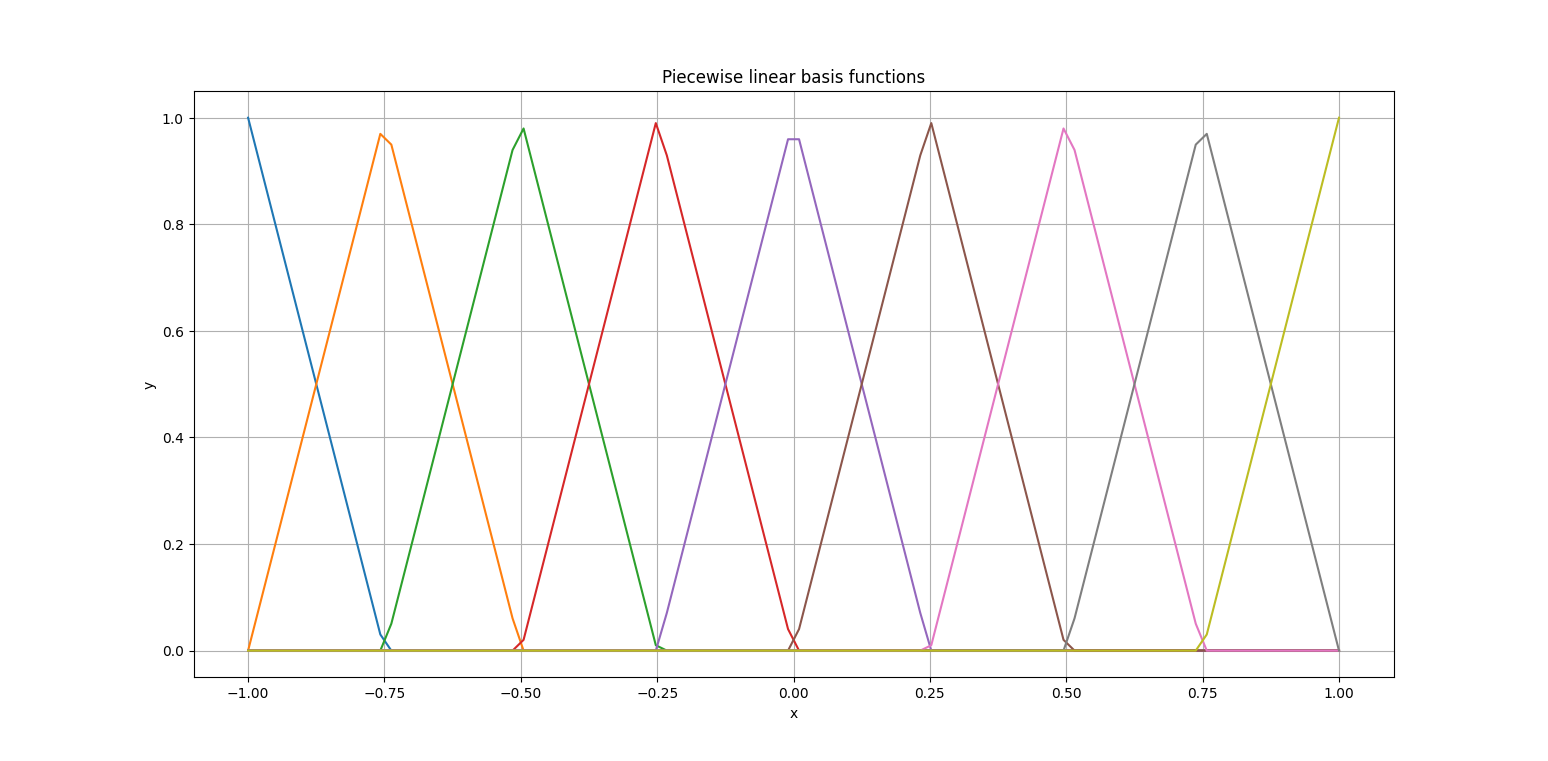
\includegraphics[width=\textwidth]{images/V_D_h.png}
    \label{fig:vd} % Etichetta per fare riferimenti nel testo
\end{figure}
\end{frame}

\begin{frame}{1d Example of \(V_h^G \) } 

\begin{figure}[htbp]
    \centering
    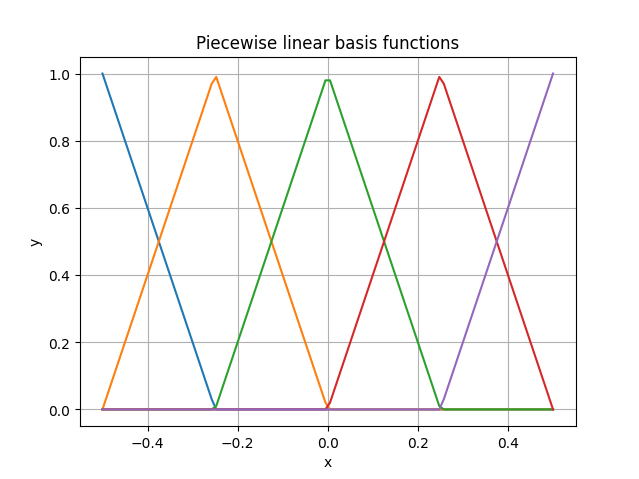
\includegraphics[width=0.7\textwidth]{images/V_G_h.png}
    \label{fig:vg} % Etichetta per fare riferimenti nel testo
\end{figure}
 
\end{frame}

\begin{frame}{1d Example of \(V_h^G \subset V_h^D\) } 

\begin{figure}[htbp]
    \centering
    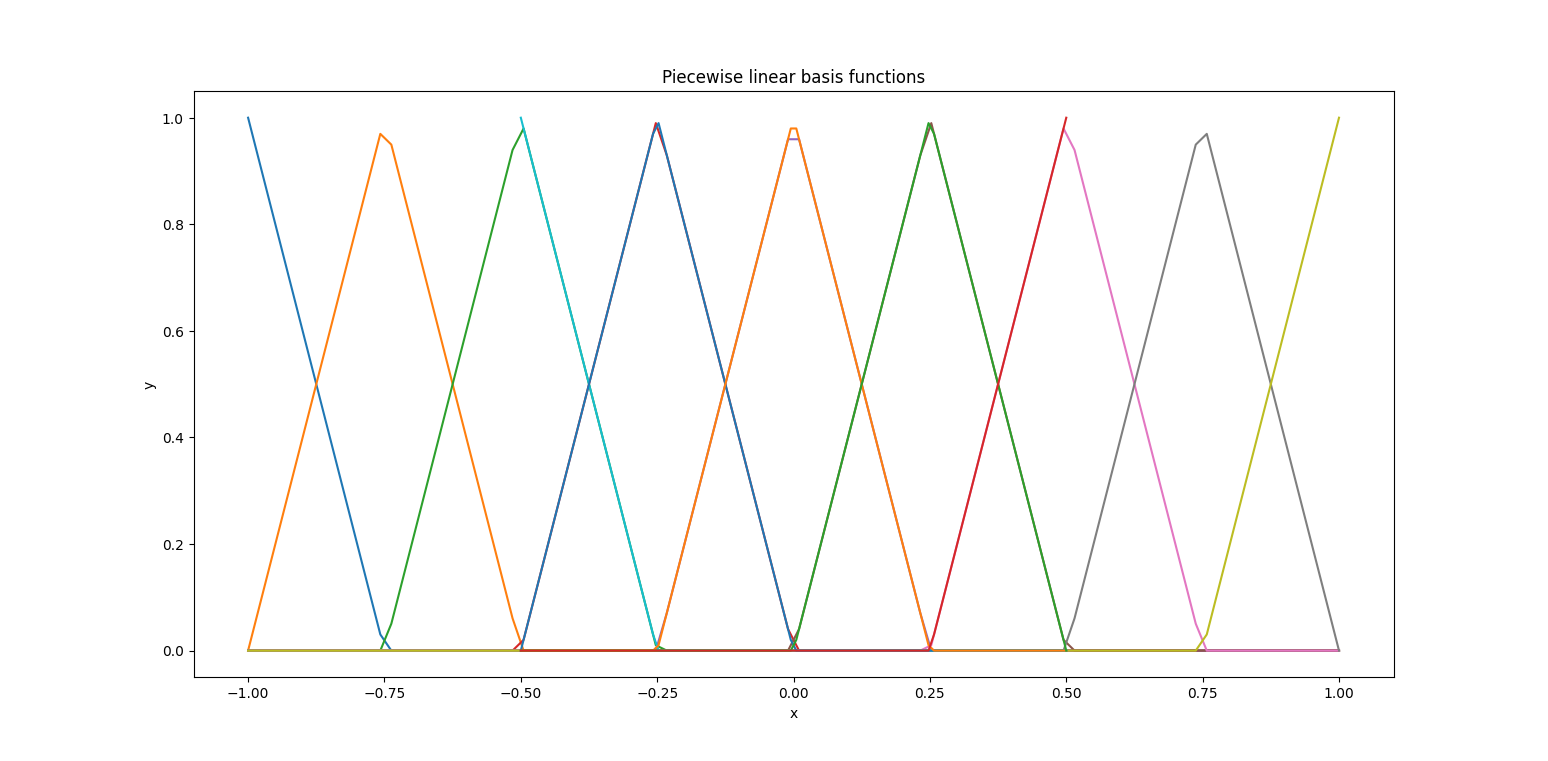
\includegraphics[width=\textwidth]{images/fem_spaces.png}
    \label{fig:vdg} % Etichetta per fare riferimenti nel testo
\end{figure}
 
\end{frame}

\begin{frame}{Solve the SPDE via FEM}
\bigskip
The discretised weak form of the SPDE reads:
\begin{equation}
  (u_h, v_h) + \kappa^{-2}(\nabla u_h, \nabla v_h) = \langle\dot{W}, v_h\rangle
  \quad \forall v_h \in V_h^D.
\end{equation}

The coefficients $\texttt{u}_i$ such that $u_h = \sum_{i=1}^m \texttt{u}_i \varphi_i$ satisfy $A\texttt{u} = b$ with:
\begin{equation}
  A_{ij} = (\varphi_i,\varphi_j) + \kappa^{-2}(\nabla\varphi_i,\nabla\varphi_j),
  \qquad
  b_i = \langle\dot{W}, \varphi_i\rangle,\quad i = 1,\ldots,m.
\end{equation}

The discretised right-hand side is Gaussian by definition of white noise:
\begin{equation}
  b \sim \mathcal{N}(0, M),\qquad M_{ij} = (\varphi_i,\varphi_j).
\end{equation}
Thus, sampling white noise reduces to sampling a Gaussian vector with \textbf{mass matrix covariance}. \textcolor{red}{ This alone does not yet improve the naive approach since an expensive global Cholesky of $M$ would still be needed.}

\end{frame}

% -----------------------------------------------------------------------

\begin{frame}{From Global to Local: Element-wise Mass Matrix}
\textcolor{green}{\textbf{Key observation:} $M$ assembles as a linear combination of element-wise matrices.}

\bigskip
For a mesh of $n$ elements with $m_e$ degrees of freedom per element:
\begin{equation}
  M = L^T \mathrm{diag}(M_e)\, L
\end{equation}
where $\mathrm{diag}(M_e)$ is block-diagonal of size $nm_e \times nm_e$, and $L$ is a
Boolean assembling matrix of size $nm_e \times m$ encoding the local-to-global map.

\bigskip
We can factorise each local mass matrix $M_e = H_e H_e^T$ and then obtain the global Cholesky factorization as
\begin{equation}
  M = L^T \mathrm{diag}(H_e H_e^T)\,L
  = \bigl(L^T \mathrm{diag}(H_e)\bigr)\bigl(L^T \mathrm{diag}(H_e)\bigr)^T
  = HH^T.
\end{equation}

With $H := L^T \mathrm{diag}(H_e)$ we can sample $b = H\mathbf{z}$, $\mathbf{z} \sim \mathcal{N}(0,I)$,
$\mathbf{z} \in \mathbb{R}^{m_e n}$, since:
\begin{equation}
  \mathbb{E}[bb^T] = H\,\mathbb{E}[\mathbf{z}\mathbf{z}^T]\,H^T = M
\end{equation}

\end{frame}

% -----------------------------------------------------------------------

\begin{frame}{Local Sampling: Algorithm and Cost}
Equivalently, we can adopt a \textbf{local sampling strategy} on each element $e$. \\
Let's consider $\mathbf{z}_e \sim \mathcal{N}(0,I)$ of length $m_e$. \\
Then:
\begin{equation}
  b = H\mathbf{z} = \sum_{e=1}^n L_e^T H_e \mathbf{z}_e = \sum_{e=1}^n L_e^T b_e,
  \qquad b_e \sim \mathcal{N}(0, M_e).
\end{equation}

The global sampling problem reduces to $n$ \textbf{independent local sampling problems} which can be immediately parallelized. \\
\bigskip

In both cases the computational cost is reduced from $\mathcal{O}(m^3)$ to $\mathcal{O}(nm_e^3)$, $m_e \ll m$.
\bigskip

Moreover, in the special case of affine linear reference element:
\[ M_e / |e| = \mathrm{const}\quad\forall\, e \]
Hence only one local Cholesky factorization is needed which drastically reduces the computational cost to $\mathcal{O}(m_e^3)$.

\end{frame}


% -----------------------------------------------------------------------

\begin{frame}{Solving Both PDEs and the Monte Carlo Estimator}
So far we have developed an efficient way to sample a white noise realization \(b(\omega)\) but to generate a single Mat\'ern random field sample we still have to:
\bigskip
\begin{enumerate}
  \item solve the SPDE: $Au_h = b(\omega)$ on $D_h$ to obtain $u_h(\cdot,\omega)$.
  \item solve the elliptic PDE with random coefficient: $\tilde{A}(\omega)\,q_h = \tilde{b}$ on $G_h$,
    with associated discrete variational formulation \[\tilde{A}_{ij} = (e^{u_h(\cdot,\omega)}\nabla\varphi_i,\nabla\varphi_j), \quad \tilde{b}_i = (1,\varphi_i), \quad i = 1, \dots, m' \quad \text{and} \ \phi_i \in V_h^G.\]
\end{enumerate}
Assuming $m \approx m'$, both PDE can be solved at a cost of $\mathcal{O}(m)$ per sample using an optimal preconditioner. \\
\smallskip

The standard unbiased Monte Carlo estimator is:
\begin{equation}
  E^{\mathrm{MC}}[\mathcal{P}] \approx E^{\mathrm{MC}}[\mathcal{P}_h]
  = \frac{1}{N}\sum_{i=1}^N \|q_h(\cdot,\omega_i)\|_{L^2(G)}
  = \frac{1}{N}\sum_{i=1}^N \sqrt{q_h(\omega_i)^T M\, q_h(\omega_i)}.
\end{equation}

This has \textbf{slow variance convergence}, making standard MC too expensive for fine meshes. 

\end{frame}

% -----------------------------------------------------------------------

\begin{frame}{Multilevel Monte Carlo}
The standard solution is to use Multilevel Monte Carlo. 
\smallskip

Consider a sequence of meshes with decreasing element diameters $\{h_l\}_{l=1}^L$. \\
The MLMC estimator is:
\begin{equation}
  E^{\mathrm{MLMC}}[\mathcal{P}_{h_L}]
  = \sum_{l=1}^{L} \frac{1}{N_l}\sum_{n=1}^{N_l}
    \Bigl(\|q_{h_l}(\omega_l^n)\|_{L^2(G)} - \|q_{h_{l-1}}(\omega_l^n)\|_{L^2(G)}\Bigr)
\end{equation}

\bigskip
The efficiency of this method relies on balancing cost and variance across levels:
\begin{itemize}
  \item \textbf{Coarse levels} ($l$ small): large variance of correction terms,
    many samples needed — but each sample is cheap (coarse mesh).
  \item \textbf{Fine levels} ($l$ large): high cost per sample — but few samples
    needed because variance of the correction $Y_l = \|q_{h_l}\| - \|q_{h_{l-1}}\|$ is small.
\end{itemize}

\end{frame}


\begin{frame}{Variance Reduction in Multilevel Monte Carlo}

We provide an intuitive explanation of the variance reduction mechanism. 

\medskip

Let
\[
Q_l := \|q_{h_l}(\omega)\|_{L^2(G)},
\qquad
Y_l := Q_l - Q_{l-1}.
\]

Then
\[
\mathrm{Var}(Y_l)
=
\mathrm{Var}(Q_l)
+
\mathrm{Var}(Q_{l-1})
-
2\,\mathrm{Cov}(Q_l,Q_{l-1}).
\]

\bigskip

The quantities $Q_l$ and $Q_{l-1}$ are computed using the same realization
$\omega$. Since $h_l$ and $h_{l-1}$ are consecutive mesh levels, the
corresponding FEM approximations are similar:
\[
u_{h_l}(\cdot,\omega)
\approx
u_{h_{l-1}}(\cdot,\omega).
\]

Assuming the quantity of interest depends continuously on the FEM solution,
\[
q_{h_l}(\cdot,\omega)
\approx
q_{h_{l-1}}(\cdot,\omega),
\]
and therefore
\[
Q_l \approx Q_{l-1}.
\]

\end{frame}


\begin{frame}{}
\bigskip

\bigskip

Hence $Q_l$ and $Q_{l-1}$ are strongly positively correlated:
\[
\mathrm{Corr}(Q_l,Q_{l-1})
=
\frac{\mathrm{Cov}(Q_l,Q_{l-1})}
{\sqrt{\mathrm{Var}(Q_l)\mathrm{Var}(Q_{l-1})}}
\approx 1,
\]
which implies
\[
\mathrm{Cov}(Q_l,Q_{l-1})
\approx
\sqrt{\mathrm{Var}(Q_l)\mathrm{Var}(Q_{l-1})}.
\]

Substituting this approximation into the variance formula,
\[
\mathrm{Var}(Y_l)
\approx
\Bigl(
\sqrt{\mathrm{Var}(Q_l)}
-
\sqrt{\mathrm{Var}(Q_{l-1})}
\Bigr)^2
\ll
\mathrm{Var}(Q_l).
\]


\end{frame}

% -----------------------------------------------------------------------

\begin{frame}{Coupled Sampling Across Levels}

The key to variance reduction is using the \textbf{same white noise realisation} on both levels $l$ and $l-1$. This means solving the SPDE on two different meshes for the same \(\omega_l^n\).

\bigskip
Let $V_{h_l}^D = \mathrm{span}(\varphi_1^l,\ldots,\varphi_{m_l}^l)$ and
$V_{h_{l-1}}^D = \mathrm{span}(\varphi_1^{l-1},\ldots,\varphi_{m_{l-1}}^{l-1})$. \\
The two discretised variational problems coupled by a common white noise sample are:
\begin{equation}
  \begin{aligned}
    (u_{h_l}, v_{h_l}) + \kappa^{-2}(\nabla u_{h_l}, \nabla v_{h_l})
      &= \langle\dot{W}, v_{h_l}\rangle(\omega_l^n)
      &&\forall\, v_{h_l} \in V_{h_l}^D \\
    (u_{h_{l-1}}, v_{h_{l-1}}) + \kappa^{-2}(\nabla u_{h_{l-1}}, \nabla v_{h_{l-1}})
      &= \langle\dot{W}, v_{h_{l-1}}\rangle(\omega_l^n)
      &&\forall\, v_{h_{l-1}} \in V_{h_{l-1}}^D
  \end{aligned}
\end{equation}
where the right-hand sides are coupled by White Noise definition: 
\[\mathbb{E}[\langle\dot{W},v^l\rangle\langle\dot{W},v^{l-1}\rangle] = (v^l, v^{l-1}).\]

The unknowns satisfy the block-diagonal linear system:
\begin{equation}
  \begin{pmatrix} A_l & 0 \\ 0 & A_{l-1} \end{pmatrix}
  \begin{pmatrix} \texttt{u}_l \\ \texttt{u}_{l-1} \end{pmatrix}
  =
  \begin{pmatrix} b_l \\ b_{l-1} \end{pmatrix}
\end{equation}

\end{frame}

% -----------------------------------------------------------------------

\begin{frame}{The Coupled Mass Matrix}

The white noise sample vector $b \in \mathbb{R}^{m_l + m_{l-1}}$ satisfies:
\begin{equation}
  b \sim \mathcal{N}(0, M), \qquad
  M = \begin{pmatrix} M_l & M_{l,l-1} \\ (M_{l,l-1})^T & M_{l-1} \end{pmatrix}
\end{equation}
where:
\[
  (M_{l,l-1})_{ij} = (\varphi_i^l, \varphi_j^{l-1}),\quad
  M_{ij} = (\varphi_i^l, \varphi_j^l),\quad
  M_{l,l-1} \in \mathbb{R}^{m_l \times m_{l-1}}
\]

\bigskip
\textbf{Challenge:} if the meshes are \textbf{non-nested}, there is no direct linear
combination that assembles $M$ element-wise, because $M_{l,l-1}$ involves inner products
of basis functions defined on \emph{different} meshes.

\bigskip
Using independent samples (off-diagonal blocks zero) would destroy the coupling and
prevent variance reduction.

\bigskip
$\Rightarrow$ Solution: construct a \textbf{super-mesh} will simplify the computation of inner product across different meshes.

\end{frame}

% -----------------------------------------------------------------------

\begin{frame}{Super-mesh: Definition and Construction}

\begin{block}{Definition 2 (Super-mesh)}
Let $D$ be a compact subset of $\mathbb{R}^d$, and let $\mathcal{T}_a, \mathcal{T}_b$ be
two tessellations of $D$. A super-mesh $\mathcal{S}$ of $\mathcal{T}_a$ and $\mathcal{T}_b$
is a common refinement of both meshes, i.e.\ a triangulation of $D$ such that:
\begin{enumerate}
  \item $\mathrm{vertices}(\mathcal{T}_a) \cup \mathrm{vertices}(\mathcal{T}_b)
        \subseteq \mathrm{vertices}(\mathcal{S})$
  \item $\mathrm{vol}(e_{\mathcal{S}} \cap e) \in \{0,\, \mathrm{vol}(e_{\mathcal{S}})\}$
        $\quad\forall\, e_{\mathcal{S}} \in \mathcal{S},\ e \in (\mathcal{T}_a \cup \mathcal{T}_b)$
\end{enumerate}
\end{block}

\end{frame}

\begin{frame}

\begin{figure}[htbp]
    \centering
    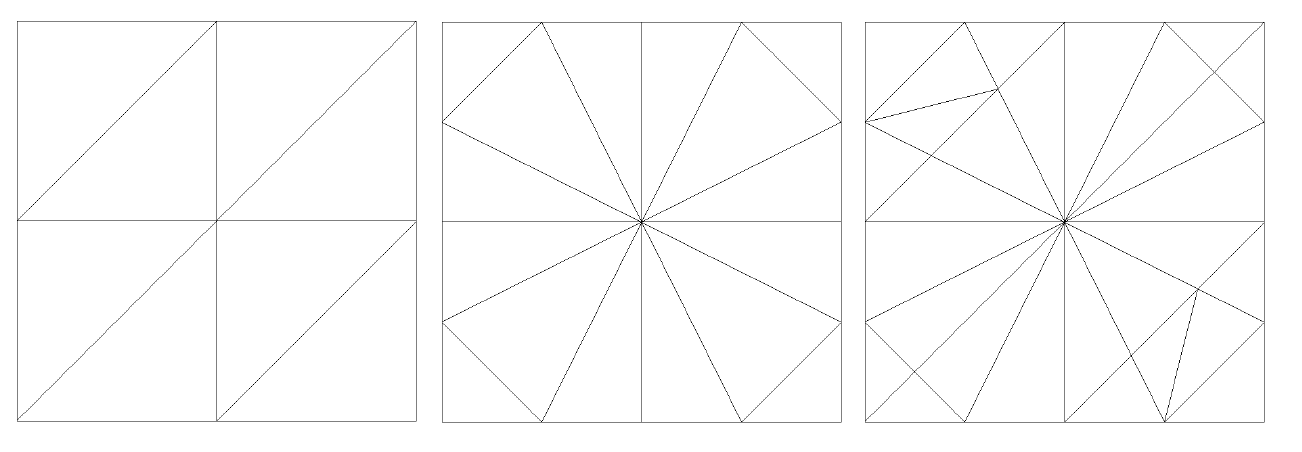
\includegraphics[height = 4.5cm, width=\textwidth]{images/supermesh.png}
    \label{fig:supermesh} % Etichetta per fare riferimenti nel testo
\end{figure}
\begin{itemize}
\item Each super-mesh element is formed by the intersection of \textbf{exactly one pair} of parent elements $e^l \in D_{h_l}$ and $e^{l-1} \in D_{h_{l-1}}$. 
\item Let $m_{e^l}$ and $m_{e^{l-1}}$ denote the number of DOFs of $V_{h_l}^D$ and $V_{h_{l-1}}^D$ restricted to those elements. Only inner products between these $m_e = m_{e^l} + m_{e^{l-1}}$ basis functions are non-zero.
\end{itemize}
\end{frame}


% -----------------------------------------------------------------------

\begin{frame}{Super-mesh Local Mass Matrix and Global Assembly}

The local mass matrix over a super-mesh element $e$ is:
\begin{equation}
  M_e = \begin{pmatrix} M_e^l & M_e^{l,l-1} \\ (M_e^{l,l-1})^T & M_e^{l-1} \end{pmatrix}
  \in \mathbb{R}^{m_e \times m_e},
  \qquad (M_e^{l,l-1})_{ij} = \int_e \varphi_i^l\,\varphi_j^{l-1}\,dx
\end{equation}

Using Boolean assembling matrices $L^l$ and $L^{l-1}$ of the two original meshes:
\begin{equation}
  M = \begin{pmatrix}(L^l)^T & (L^{l-1})^T\end{pmatrix}
  \begin{pmatrix}
    \mathrm{diag}(M_e^l) & \mathrm{diag}(M_e^{l,l-1}) \\
    \mathrm{diag}(M_e^{l,l-1})^T & \mathrm{diag}(M_e^{l-1})
  \end{pmatrix}
  \begin{pmatrix}L^l \\ L^{l-1}\end{pmatrix}
  = \begin{pmatrix} M_l & M_{l,l-1} \\ (M_{l,l-1})^T & M_{l-1} \end{pmatrix}
\end{equation}

\bigskip
This gives the desired linear assembling of the coupled mass matrix and the \textbf{same efficient local sampling technique} now applies. \\

\end{frame}

% -----------------------------------------------------------------------

\begin{frame}{Assembling the Coupled Sample}

For each super-mesh element $e$, draw $b_e \sim \mathcal{N}(0, M_e)$ and split
$b_e = ((b_e^l)^T\; (b_e^{l-1})^T)^T$.  \\ By construction:
\begin{equation}
  b_e^l \sim \mathcal{N}(0, M_e^l),\quad
  b_e^{l-1} \sim \mathcal{N}(0, M_e^{l-1}),\quad
  \mathbb{E}[b_e^l (b_e^{l-1})^T] = M_e^{l,l-1}
\end{equation}

Using the Boolean matrices, for each super-mesh element $e$:
\begin{equation}
  b^l = \sum_{e=1}^n (L_e^l)^T b_e^l,
  \qquad
  b^{l-1} = \sum_{e=1}^n (L_e^{l-1})^T b_e^{l-1}
\end{equation}
where $n$ is the number of super-mesh elements.

This enforces the correct distribution since sums of Gaussian random variables are Gaussian.
In particular:
\begin{equation}
  \mathbb{E}[b^l (b^l)^T]
  = \sum_{i,j} (L_i^l)^T \mathbb{E}[b_i^l (b_j^l)^T] L_j^l
  = \sum_i (L_i^l)^T M_i^l\, L_i^l
  = (L^l)^T \mathrm{diag}(M_i^l)\, L^l = M_l
\end{equation}
and analogously for $l-1$ and the mixed term giving $M_{l,l-1}$.

\end{frame}

% -----------------------------------------------------------------------

\begin{frame}{Lemma: Affine Reference Element}

\begin{block}{Lemma 1}
Let $V_{h_l}^D$, $V_{h_{l-1}}^D$ be two FEM spaces over tessellations $D_{h_l}$,
$D_{h_{l-1}}$ of $D$. Let $\mathcal{S}$ be a super-mesh, $e \in \mathcal{S}$.
Assume $V_{h_{l-1}}^D|_e \subseteq V_{h_l}^D|_e$ (nested restrictions) and $M_e^l$
non-singular. Then:
\begin{itemize}
  \item $\mathrm{rank}(M_e) = \mathrm{rank}(M_e^l)$ and
    $M_e^{l-1} = (M_e^{l,l-1})^T (M_e^l)^{-1} M_e^{l,l-1}$
\end{itemize}
If the transformation to the reference element is affine and $V^S|_e$ is a FEM subspace
over $\mathcal{S}$, with $V_{h_{l-1}}^D|_e,\, V_{h_l}^D|_e \subseteq V^S|_e$, then there
exist local interpolation matrices $R_e^l$ and $R_e^{l-1}$ such that:
\begin{itemize}
\item \begin{equation}
  M_e^l = (R_e^l)^T M_e^S R_e^l,\quad
  M_e^{l-1} = (R_e^{l-1})^T M_e^S R_e^{l-1},\quad
  M_e^{l,l-1} = (R_e^l)^T M_e^S R_e^{l-1}
\end{equation}
\end{itemize}
\end{block}

\end{frame}

\begin{frame}


\bigskip
\begin{itemize}
\item In practice for Lagrange FEM we can assemble the element-wise samples as:
\begin{equation}
  b_e^k = (R_e^k)^T H_r\, |e_r|^{-1/2} |e|^{1/2}\, \mathbf{z}_e,
  \quad \mathbf{z}_e \sim \mathcal{N}(0,I),\quad k \in \{l-1,\,l\}
\end{equation}
where $M_e^S / |e| = H_r H_r^T / |e_r| = \mathrm{const}$ is the Cholesky factorisation over the reference element $e_r$. 
\item As in the non coupled case the Cholesky factorization $H_r$ is computed \textbf{only once}.
\end{itemize}
\end{frame}

\begin{frame}{\strut}
    \vfill
    \begin{center}
        {\Huge\bfseries\color{blue} Questions? \par}
    \end{center}
    \vfill
\end{frame}


% -----------------------------------------------------------------------
\section{1D Numerical Implementation}
% -----------------------------------------------------------------------

\begin{frame}{1D Numerical Experiments: Monte Carlo Implementation}

We aim to replicate the results shown in the article in the \textbf{simpler 1D case}. This allows us to focus on the main ideas rather than the more complex FEM reasoning which is beyond the scope of the seminar. 
\bigskip

The code is available: \href{https://github.com/fede-mat/mlmc_fem_1d_solver}{\faGithub\ mlmc\_fem\_1d\_solver}.

\bigskip
\textbf{Setup:}
\begin{itemize}
  \item Domains: $G = [-0.5,\,0.5]$ and $ D = [-1,\,1]$ with \(h = 1/100\).
  \item FEM function space: piecewise linear test function (Lemma holds).
  \item Mat\'ern covariance with $\kappa=10$.
  \item Quantity of interest: $ \mathbb{E}[\mathcal{P}] \approx \mathbb{E}[\|q_h\|_{L^2(G)}] $ .
  \item $N = 100$, $N = 1\,000$ and  $N = 10\,000$  
\end{itemize}

\end{frame}

\begin{frame}{1D Results: Distribution and Convergence - 100 samples}

\begin{figure}[htbp]
    \centering
    % Prima immagine (49% della larghezza del testo)
    \begin{minipage}[b]{0.49\textwidth}
        \centering
        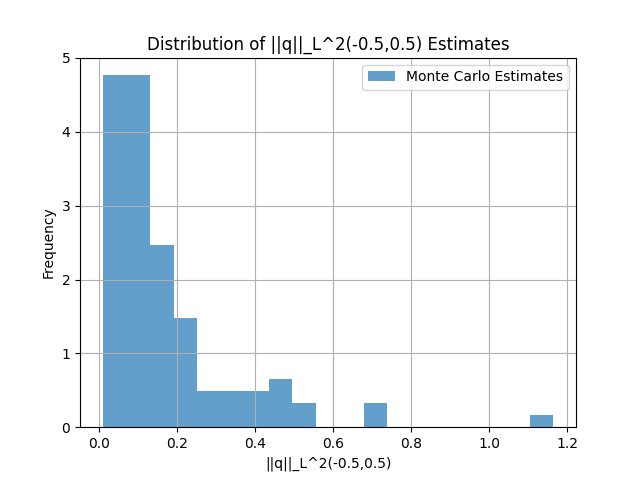
\includegraphics[height=4.5cm,width=\textwidth]{../../results/histogram_mc_estimates_seed_2026_samples_100.png}
    \end{minipage}% <--- Nota questo percento, elimina spazi spuri
    \hfill % Spazio minimale tra le due foto
    % Seconda immagine (49% della larghezza del testo)
    \begin{minipage}[b]{0.49\textwidth}
        \centering
        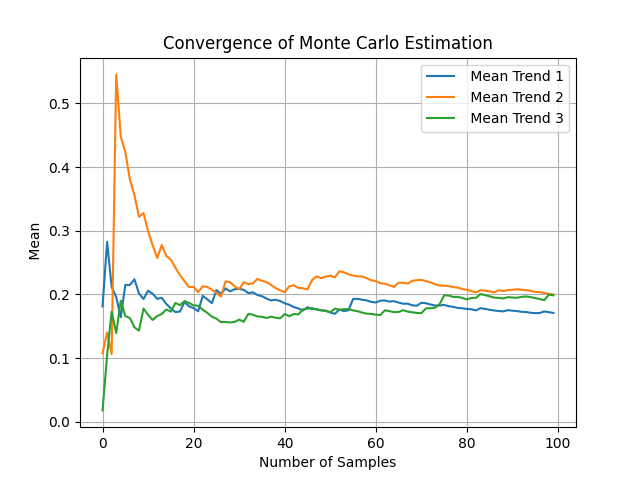
\includegraphics[height=4.5cm,width=\textwidth]{../../results/convergence_mc_seed_2026_samples_100.png}
    \end{minipage}
    
    \vspace{-2mm} % Riduce lo spazio bianco sotto le foto
    \label{fig:conv_comparison}
\end{figure}

\begin{center}
{\small
\texttt{Estimated expected value of ||q||\_L\textasciicircum2(-0.5,0.5) using Monte Carlo with 100 samples, seed 2026: 0.17095288589067742.} \\
\texttt{Time taken for Monte Carlo estimation: 0.0 hours 0 min 8.39 seconds.}}
\end{center}

\end{frame}

% -----------------------------------------------------------------------

\begin{frame}{1D Results: Distribution and Convergence - 1000 samples} 

\begin{figure}[htbp]
    \centering
    % Prima immagine (49% della larghezza del testo)
    \begin{minipage}[b]{0.49\textwidth}
        \centering
        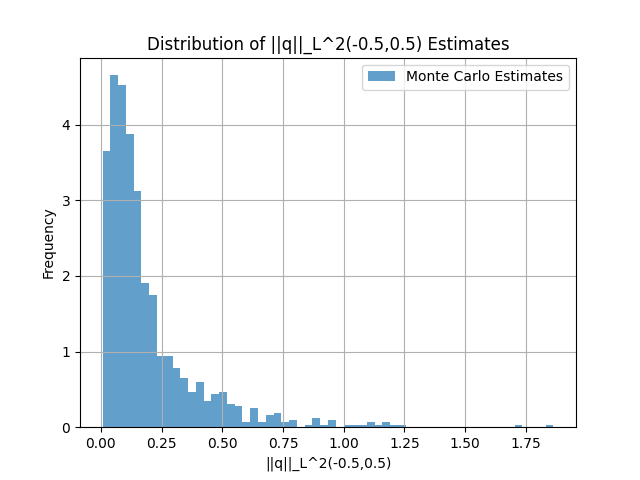
\includegraphics[height=4.5cm,width=\textwidth]{../../results/histogram_mc_estimates_seed_2026_samples_1000.png}
    \end{minipage}% <--- Nota questo percento, elimina spazi spuri
    \hfill % Spazio minimale tra le due foto
    % Seconda immagine (49% della larghezza del testo)
    \begin{minipage}[b]{0.49\textwidth}
        \centering
        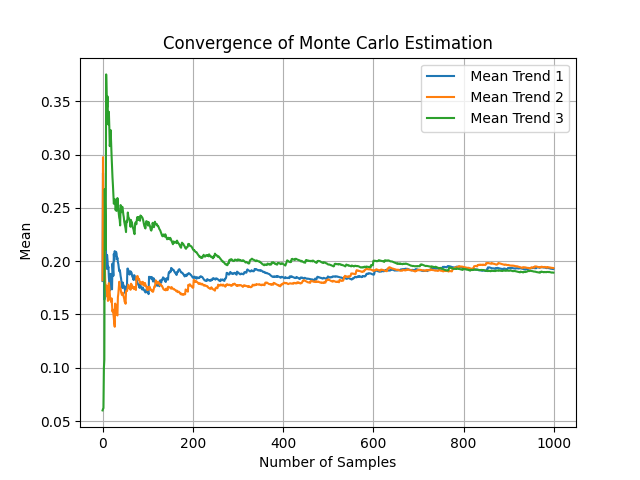
\includegraphics[height=4.5cm,width=\textwidth]{../../results/convergence_mc_seed_2026_samples_1000.png}
    \end{minipage}
    
    \vspace{-2mm} % Riduce lo spazio bianco sotto le foto
    \label{fig:conv_comparison}
\end{figure}

{\small \begin{center}
\texttt{Estimated expected value of ||q||\_L\textasciicircum2(-0.5,0.5) using Monte Carlo with 1000 samples, seed 2026: 0.19263251472509055.} \\
\texttt{Time taken for Monte Carlo estimation: 0.0 hours 1 min 18.32 seconds.}
\end{center}
}
\end{frame}

\begin{frame}{1D Results: Distribution and Convergence - 10000 samples}

\begin{figure}[htbp]
    \centering
    % Prima immagine (49% della larghezza del testo)
    \begin{minipage}[b]{0.49\textwidth}
        \centering
        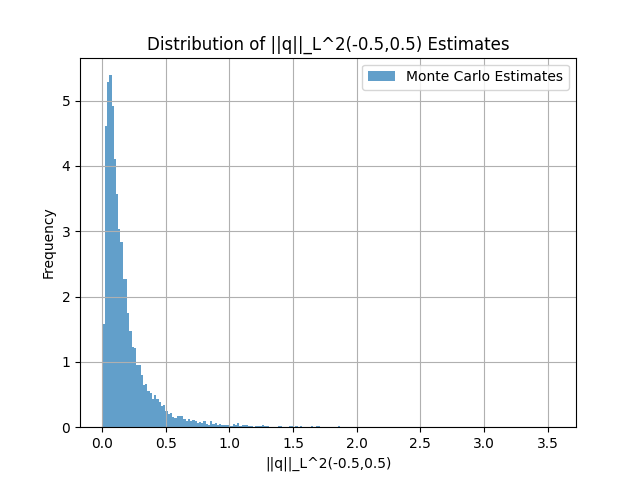
\includegraphics[height=4.5cm,width=\textwidth]{../../results/histogram_mc_estimates_seed_2026_samples_10000.png}
    \end{minipage}% <--- Nota questo percento, elimina spazi spuri
    \hfill % Spazio minimale tra le due foto
    % Seconda immagine (49% della larghezza del testo)
    \begin{minipage}[b]{0.49\textwidth}
        \centering
        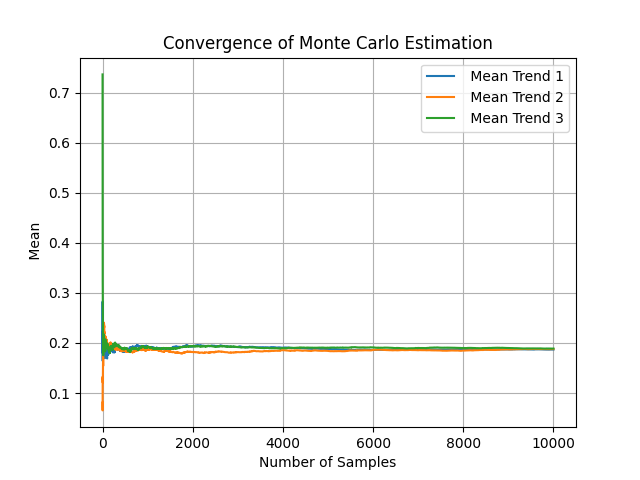
\includegraphics[height=4.5cm,width=\textwidth]{../../results/convergence_mc_seed_2026_samples_10000.png}
    \end{minipage}
    
    \vspace{-2mm} % Riduce lo spazio bianco sotto le foto
    \label{fig:conv_comparison}
\end{figure}

{\small \begin{center}
\texttt{Estimated expected value of ||q||\_L\textasciicircum2(-0.5,0.5) using Monte Carlo with 10000 samples, seed 2026: 0.18688853989513146.} \\
\texttt{Time taken for Monte Carlo estimation: 0.0 hours 8 min 14.11 seconds.}
\end{center}
}
\end{frame}

% ----------------------------------------------------------------------- 

\begin{frame}{1D Numerical Experiments: Multilevel Monte Carlo Implementation}


\bigskip
\textbf{Setup:}
\begin{itemize}
  \item Domains: $G = [-0.5,\,0.5]$ and $ D = [-1,\,1]$ with \(h = 1/100\).
  \item FEM function space: piecewise linear test function (Lemma holds).
  \item Mat\'ern covariance with $\kappa=10$.
  \item Levels: \( l = 1 , \dots , 10 \) with \( h_l = \frac{1}{l  \cdot 10}\)
  \item The number of samples for each level computed as an empirical approximation of theoretical optimal one, i.e. \( M_l = \sqrt{\frac{\mathbb{V}[Y_l]}{\text{Cost}(Y_l)}}. \)

  \item Quantity of interest: $ \mathbb{E}[\mathcal{P}] \approx \mathbb{E}[\|q_h\|_{L^2(G)}] $ .
  \item $N = 100$, $N = 1\,000$ and  $N = 10\,000$  
\end{itemize}

\textbf{Warning:} I tried my best to implement MLMC method but there might be some minor issues.

\end{frame}

\begin{frame}{1D Results: Distribution and Convergence - 100 samples}

\begin{figure}[htbp]
    \centering
    	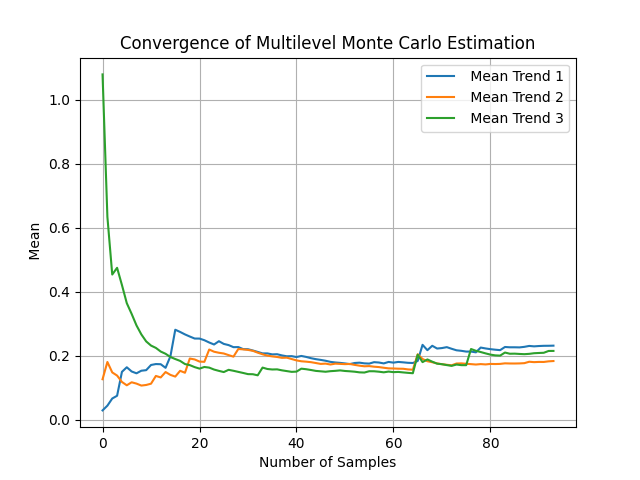
\includegraphics[height=4.5cm]{../../results/convergence_mlmc_seed_2026_samples_100.png}
    \label{fig:mlmc_100}
\end{figure}

\begin{center}
\small
\texttt{Estimated expected value of ||q||\_L\^{}2(-0.5,0.5) using Multilevel Monte Carlo with 100 samples, seed 2026: 0.2311756059521551.} \\
\texttt{Time taken for Multilevel Monte Carlo estimation:\\ 0.0 hours 0 min 1.32 seconds.}
\end{center}


\end{frame}

% -----------------------------------------------------------------------

\begin{frame}{1D Results: Distribution and Convergence - 1000 samples} 

\begin{figure}[htbp]
    \centering
    	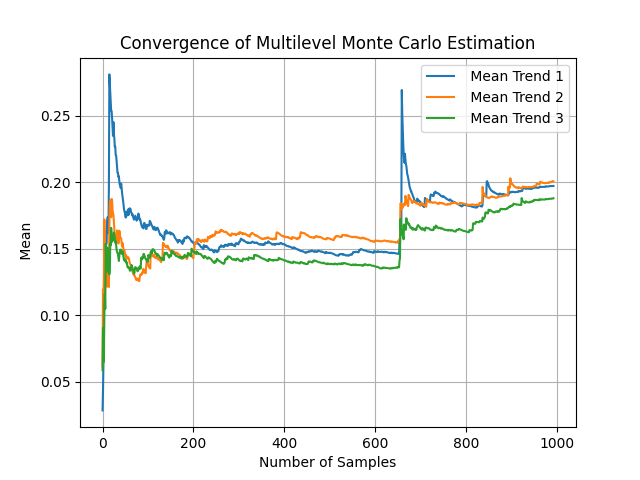
\includegraphics[height=4.5cm]{../../results/convergence_mlmc_seed_2026_samples_1000.png}
    \label{fig:mlmc_1000}
\end{figure}

\begin{center}
\small
\texttt{
Estimated expected value of ||q||\_L\^{}2(-0.5,0.5) using Multilevel Monte Carlo with 1000 samples, seed 2026: 0.19719679131929285 \\
Time taken for Multilevel Monte Carlo estimation: \\ 0.0 hours 0 min 12.68 seconds}
\end{center}

\end{frame}

\begin{frame}{1D Results: Distribution and Convergence - 10000 samples}

\begin{figure}[htbp]
    \centering
    	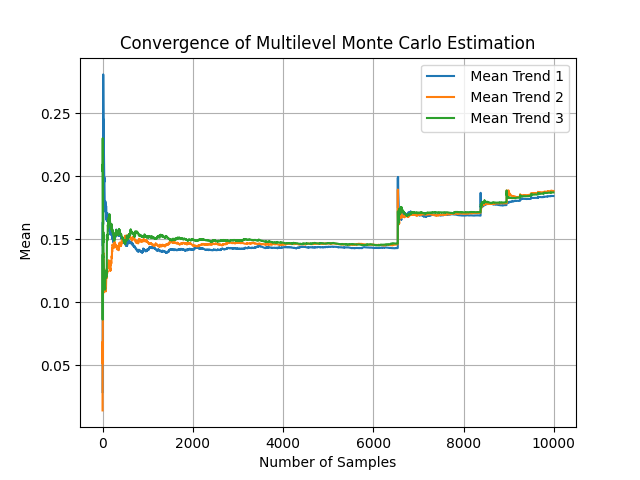
\includegraphics[height=4.5cm]{../../results/convergence_mlmc_seed_2026_samples_10000.png}
    \label{fig:mlmc_10000}
\end{figure}

\begin{center}
\small
\texttt{
Estimated expected value of ||q||\_L\^{}2(-0.5,0.5) using Multilevel Monte Carlo with 10000 samples, seed 2026: 0.184344711791526 \\
Time taken for Multilevel Monte Carlo estimation: \\0.0 hours 2 min 26.69 seconds}
\end{center}

\end{frame}

% -----------------------------------------------------------------------
\section{Conclusion}
% -----------------------------------------------------------------------

\begin{frame}{Discussion}

\textbf{Main advantage:}
\begin{itemize}
  \item[\textbullet] The local, element-wise structure of the sampling procedure
    leads to a \textbf{straightforwardly parallelisable} implementation.
\end{itemize}

\bigskip
\textbf{Main drawback:}
\begin{itemize}
  \item[\textbullet] Generating each sample for both Monte Carlo and Multilevel Monte Carlo
    requires \textbf{solving two PDEs} to obtain a single realisation for estimating the
    desired quantity.
\end{itemize}    

\end{frame}

\end{document}